\documentclass[a4paper,12pt]{article}
%\usepackage{ngerman}
\usepackage{soul}
\usepackage{mathtools}
\usepackage{amssymb,amsmath,amsfonts}
\usepackage{cancel}
\usepackage[utf8]{inputenc}
\usepackage{graphicx}
\usepackage{geometry}
\usepackage[autostyle=true,german=quotes]{csquotes}
\usepackage{gensymb}
\usepackage{units}
\usepackage{fancyhdr}
\usepackage[nottoc,numbib]{tocbibind}
\usepackage{abstract}
\usepackage[font=small,labelfont=bf]{caption}
\usepackage[
citestyle=numeric
]{biblatex}

\addbibresource{./../lib/lib.bib}
\graphicspath{{./../figures/}}

\geometry{a4paper, left=25mm, right=25mm, top=20mm, bottom=20mm}

\pagestyle{plain}
%\pagestyle{fancy}
%\lhead{Left header}
%\rhead{Right header}
%\lfoot{left footer}
%\rfoot{right footer}

\renewcommand{\abstractname}{Summary}

\title{SOLENSIM Model summary}


\author{Anton Douginets (anton.douginets@physik.hu-berlin.de)
	\and
	Andrii Yanovets (yanoveta@hu-berlin.de)}

\date{\today}

\begin{document}

\thispagestyle{empty}
\maketitle

\begin{abstract}
This is a summarizing description of the physical model - i.e. axial field calculation, characteristic value determination from axial field, field integrals etc.
\end{abstract}

\tableofcontents

\newpage

\pagenumbering{arabic}

\section{Chromatic aberrations and focal spot size}

\begin{figure}
  \centering
  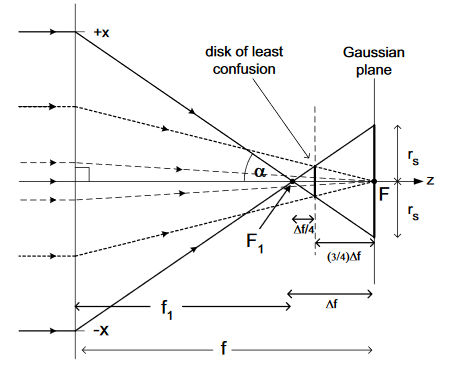
\includegraphics[width=0.75\textwidth]{cs_illustration}
  \caption{title}
\end{figure}

\[
1/f=const.\cdotp F2
\]

\[
\triangle f\simeq c\cdotp x^{2}
\]

\[
x=f_{1}tan\left(\alpha\right)\simeq f\cdotp tan\left(\alpha\right)
\]

\[
r_{s}=\triangle f\cdotp tan\left(\alpha\right)\simeq\triangle f\cdotp\alpha\approx\left(c\left(f\cdotp tan\left(\alpha\right)\right)^{2}\right)\cdotp tan\left(\alpha\right)=C_{s}tan\left(\alpha\right)^{3}=C_{s}\cdotp\left(\frac{max\left\{ x\right\} }{f-\triangle f}\right)^{3}
\]

\[
\underset{f\approx f_{1}}{=}C_{s}\cdotp\left(\frac{max\left\{ x\right\} }{f}\right)^{3}\quad(1)
\]

If $f\cancel{\approx}f_{1}$then replace $f$ in (1) with $f-max\left\{ x\right\} ^{2}\cdotp\frac{C_{s}}{f^{2}}$

\printbibliography

%\section{Appendix}
%Also as begin/end environment
%\listoffigures

%\listoftables

\end{document}
